\documentclass[a4paper, 12pt]{article}
\usepackage{lipsum}
\usepackage{layout}
\usepackage[margin=72pt]{geometry}
\usepackage{graphicx}
\usepackage{amssymb}
\usepackage{amsmath}
\pagestyle{empty} 
%\usepackage{verbatimbox}
\usepackage{fancyvrb}
\usepackage{spverbatim}
\usepackage{mathtools}
\usepackage{float}
\pagestyle{plain}
%--------------------------------------------------------------------------------------------------------------------------------------------------------------------
\begin{document}
\begin{titlepage}
\begin{center}
\Large\underline{MATH49111 - Scientific Computing:   Project 1}\\
\end{center}
\begin{center}
\large\underline{Project 4 - Sorting Algorithms}
\end{center}
Name: Tom Cantrell\\
Student ID: 10170539\\
\end{titlepage}

\tableofcontents
\newpage
\section{Introduction}
Searching through a list, vector or array of data and then sorting its contents is an extremely common problem, which can be solved by using an ever-growing number of algorithms of varying complexity. Fundamentally a sorting algorithm is an algorithm which arranges objects in an array into a specific order. In this report we will consider numerical order, where lists sorted in ascending order are desirable. This however can be extended to any desired order whether it be numerical descending or alphabetical order. \\

The sorting algorithms discussed in this report are bubblesort, quicksort and heapsort, these sorting algorithms are all comparison sorts, that is these algorithms sort the elements of a vector by comparing the size or magnitude of the elements themselves. 

\subsection{Initialising a random list}
In order to produce vectors of a specified length that have random entries we can appeal to the function rand(). This is a pseudo-random number generator which produces the same values each time the program is run. However seeding the generator at the beginning of the main() function we are able to produce different random numbers each time the function is called to produce a pseudo-random number. \\

Creating our initial data, we add the following member function to our MVector class specified in the question,
\begin{verbatim}
void initialise_random(double xmin, double xmax)	{
	size_t s = v.size();
	for (size_t i = 0; i < s; i++)
	{
		v[i] = xmin + (xmax - xmin) * rand() / static_cast<double>(RAND_MAX);
	}
}
\end{verbatim} 
Now, testing this function we can produce a vector which takes entries randomly from a predetermined interval. For example defining the interval as $[-a,a]$ for $a>0$, we would expect to see equally as many negative numbers produced as positive. The following output shows a vector of length 10, with values randomly selected from the interval $[-1000000.0,1000000.0]$.
\begin{spverbatim}
630116 606067 -293680 -132847 361980 858821 -314737 472518 657704 421369
\end{spverbatim} 
As we know these are only pseudo-random numbers, which although they are sufficient for the sorting algorithms (which is all they will be used for here), these are possibly of rather low quality. Moreover, it's important to investigate how random these pseudo-random numbers are, thereby ensuring there are no disernible patterns or regularities in the way these numbers are produced.\\

In an attempt to test for randomness, or at least visualise the distribution of the pseudo-random numbers, we can create a plot to illustrate the uniformity of the data.  
\begin{figure}[H]
\centering
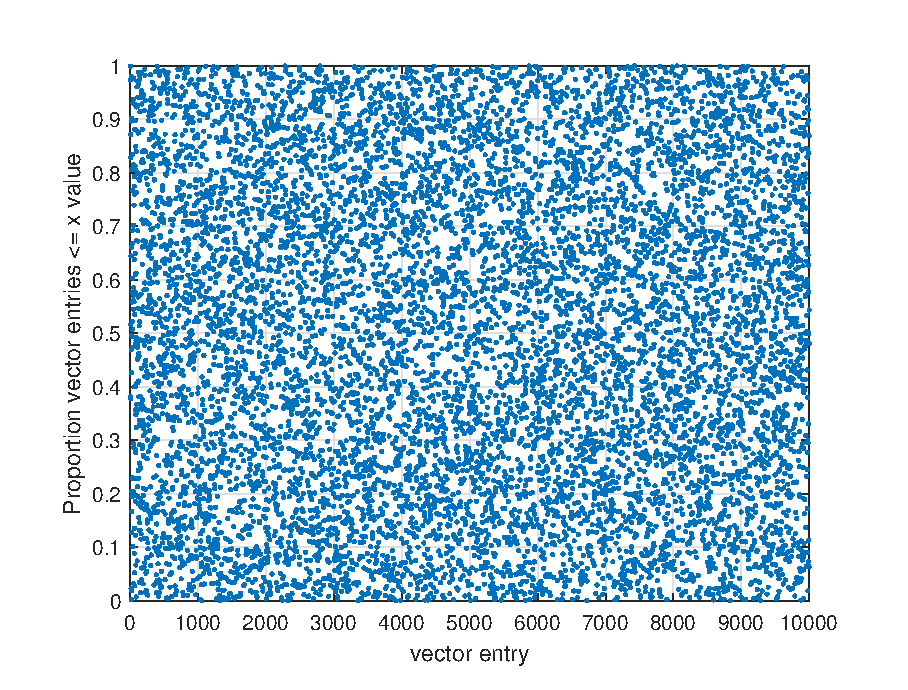
\includegraphics[scale=0.75]{test_random1}
\end{figure}
To create this plot, a vector was given 10,000 pseudo-random entries from the interval $[-1000000.0,1000000.0]$. Then for each entry, a simple program loops over the vector counting how many other entries are less than or equal to that entry, this value is then divided by the number of entries. These values are then plotted.\\

As we can see from the figure the distrubtion appears to be random, as there do not appear to be any patterns or regularities in the plot. It is known that pseudo-random numbers are never truly random however from simply visualising the distribution this way, the numbers produced do appear random. In order to test the randomness more thoroughly, one could conduct some statistical analysis on the distribution of a larger set of randomly produced entries. \\

\section{Formulation of the sorting algorithms}
\subsection{Bubblesort}

Bubblesort is a very simple sorting algorithm, which starts at the beginning of the vector and then compares the first element with the second element. If the first element is greater than the second, they are swapped otherwise the list is not altered and the algorithm moves on to comparing the second with the third and so on. Hence by the end of the first pass of the whole vector, the greatest element in the vector will be at the end. More passes and swaps are made until the vector is sorted. \\

A hard-copy of the function bubble(...):
% Bubblesort hard-copy
\begin{spverbatim}
void bubble(MVector& v)
{
	int stop = 1;
	while (stop < v.size()) // loop over the vector until stopping condition is reached
	{
		stop = 1;
		for (int i = 0; i < (v.size() - 1); i++) 
		{
			if (v[i] > v[i + 1]) // Comparing adjacent elements
			{
				v.swap(i, i + 1); 
				stop--;
			}
			else { stop++; }
		}
	}
}
\end{spverbatim}


\subsubsection{Results}

\underline{Test cases}\\

Conducting some simple test cases with some randomly initialised lists, we can test the validity of the source code above. The source code that produces these test cases can be found in the appendix.\\ 
Output:
\begin{spverbatim}
-65587.3 -10379.3 81658.4 -23758.7 49461.3 51719.7 570.696 -77007.4 41282.4 -47679.1
Using bubblesort algorithm:
-77007.4 -65587.3 -47679.1 -23758.7 -10379.3 570.696 41282.4 49461.3 51719.7 81658.4
\end{spverbatim}
\begin{figure}[H]
\centering
\includegraphics[scale = 0.75]{Bubblesort_average_time}
\caption{Average sort time for bubblesort algorithm with $n$ increasing.}
\end{figure}

\begin{table} [H]
\centering
\begin{tabular}{ c | c | c}
$n$ & Average sort time (milliseconds)  & ratio of sort time \\ \hline
         2      &       0.00075  & -\\
         4       &      0.00226 & 3.0133 \\
         8        &     0.01059 & 4.6858 \\
        16        &     0.03443 & 3.2512\\
        32        &     0.14257 &  4.1409\\
        64         &    0.52521 & 3.6839\\
       128        &     2.28044 & 4.3420\\
       256        &     9.58698 & 4.2040 \\
       512        &     37.1824 & 3.8784\\
      1024       &      149.427 & 4.0188\\
      2048       &      598.006 & 4.0020\\
      4096       &      2322.04 & 3.8830 \\
      8192       &      9509.97 & 4.0955 \\
\end{tabular}
\caption{Average sort time in milliseconds for the bubblesort algorithm for a vector of length $n$.}
\end{table}
In order to more easily see the order of complexity produced by the source code shown above in the hard-copy of bubblesort algorithm, we increase the length of the vector by a factor of two. The average sort time is then found by timing ten randomly initialised vectors of a given length and computing the sum of these times and then dividing by ten. \\

The average performance of bubblesort is $O(n^2)$ with $O(n^2)$ swaps , this is also the worst case performance of the bubblesort algorithm. The best-case performance is however $O(n)$ with $O(1)$ swaps \cite{BlackPE}. From the data shown in table 1 we can see that this particular implementation of bubblesort has achieved $O(n^2)$ complexity therefore achieving at best average performance. As the length of the vector $n$ increases by a factor of two, if we have $O(n^2)$ order of complexity then in doubling the number of elements in the vector we should expect to see the average sort time quadruple. \\

This is illustrated in table 1 in the third column. The third column shows the ratio of the average sort times between vectors that differ by a factor of two (the third column is the ratio of the current average sort time and the previous which does not exist for $n=2$, hence the hyphen in the first entry of the column). For the relatively small values of $n$ we see that this ratio fluctuates around the value 4, however for $n>512$ we see that this ratio appears to converge to a value of 4, only deviating slightly by at most 0.117 when the ratio is equal to 3.8830. Hence this confirms the complexity of bubblesort using the implementation specified in the source code above is $O(n^2)$.\\

In this case, as we have at best average performance with complexity of $O(n^2)$, a factor of four appears in the average sort time between vectors that differ by a factor of two. However if the algorithm had achieved the complexity corresponding to best-case performance, $O(n)$, then for vectors differing by a factor of two we should expect to see the average sort time differ by a factor two also.     


% A hard-copy of function bubble(....)
% A graph of the average sort time as a fn of n.  Function form of curve?
% Analysis of expected form of curve from theoretical considerations i.e whats the complexity of the algorithm
\subsection{Quicksort}

Quicksort is slightly more complex than bubblesort as it employs partitioning as a means of sorting the vector of elements into sections which are then themselves sorted into subsections and sorted by partitioning and so on. This is where recursion can be introduced to speed up the algorithm as the quicksort algorithm is applied to subsections.\\ 

The algorithm begins by randomly selecting an element from the vector and denotes this as the pivot, then the elements to the left and right of the pivot are compared with the pivot and if their value is less than the pivot it places them to the left of the pivot and to the right of the pivot if their value is greater than pivot. This is then applied to the subsections of the vector created and is repeated on successive subsections until subsections are of length one, that is there are not any more elements to sort. This is our termination condition, if there are only subsections of length one or zero, we should just return the vector as it is now sorted. 
    
A hard-copy of the function quick{\_}recursive:
% quick_recursive hard-copy
\begin{spverbatim}
void quick_recursive(MVector& v, int start, int end)
{
	int x = start + (end - start) * static_cast<double>(rand()) / static_cast<double>(RAND_MAX); // random pivot
	MVector s1, s2, s3;
	double pivotvalue = v[x];
	for (int j = 0; j <= end; j++) // create vectors s1, s2 and s3
	{
		if (v[j] < v[x]) { s1.push_back(v[j]); }
		else if (v[j] == v[x]) { s2.push_back(v[j]); }
		else { s3.push_back(v[j]);}
	}
	// Call fn recursively
	if (s3.size() > 1)
	{
		quick_recursive(s3, 0, s3.size()-1);
	}
	if (s1.size() > 1)
	{
		quick_recursive(s1, 0, s1.size()-1);
	}
	for (int k = start; k < start + s1.size(); k++) // add the sorted sub-vectors back to main vector
	{
		v[k] = s1[k - start];
	}
	for (int k = start + s1.size(); k < start + s1.size() + s2.size(); k++)
	{
		v[k] = s2[k - s1.size() - start];
	}
	for (int k = start + s1.size() + s2.size(); k < start + s1.size() + s2.size() + s3.size(); k++)
	{
		v[k] = s3[k - s1.size() - s2.size() - start];
	}
}
\end{spverbatim}

\subsubsection{Results}

\underline{Test cases}\\

Conducting some simple test cases with some randomly initialised lists, the validity of the source code above is tested. Source code that produces these test cases can be found in the appendix.\\ 
Output:
\begin{spverbatim}
-46195.9 48533.6 57756.3 77153.8 -3988.77 53453.2 -96563.6 -6503.49 -17532.9 546.281
 Using quicksort algorithm:
-96563.6 -46195.9 -17532.9 -6503.49 -3988.77 546.281 48533.6 53453.2 57756.3 77153.8
\end{spverbatim}
\begin{figure}[H]
\centering
\includegraphics[scale = 0.75]{Quicksort_average_time}
\caption{Average sort time for quicksort with $n$ increasing.}
\end{figure}

Similar to bubblesort, quicksort has a worst-case time complexity of $O(n^2)$ however the average-case and best-case time complexity has time complexity of $O(n\log(n))$ \cite{GueronKrasnov}. From this, we can show what we expect to happen with the average sort time. Suppose we have a vector of length $n$, from the analysis done on the average sort time of bubblesort, we already can expect the average sort time to quadruple if the length of the vector doubles to $2n$, if we have time complexity of $O(n^2)$. Now, suppose we have time complexity of $O(n\log(n))$, doubling the length of the vector to $2n$ has the following effect on average sort time,
\begin{center}
$2n\log(2n) = 2n(\log(n) + \log(2)) = n\log(n)\left[ \frac{2\log(2)}{\log(n)} + 2\right].$
\end{center} 
\begin{table}[H]
\centering
\begin{tabular}{ c | c | c | c }
$n$ & Average sort time (milliseconds) & Ratio of average sort time & Theoretical factor \\ \hline
         2     &       0.006677 & - & - \\
         4      &      0.016704 &2.5017& 3.0000\\
         8       &     0.046272 &2.7701& 2.6667\\
        16      &      0.130234 & 2.8145& 2.5000\\
        32      &      0.294255 &2.2594& 2.4000 \\
        64      &      0.632575 &2.1498 & 2.3333\\
       128     &        1.35098 & 2.1357  &2.2857\\
       256     &        2.88328 & 2.1342  &2.2500 \\
       512     &        6.47135 & 2.2444 & 2.2222\\
      1024     &        12.9754 &2.0051 & 2.2000\\
      2048     &        28.4203 & 2.1903 & 2.1818\\
      4096      &       58.8226 &2.0697 & 2.1667\\
      8192      &        122.62 &2.0846 & 2.1538\\
\end{tabular}
\caption{Average sort time in milliseconds for the quicksort algorithm for a vector of length $n$.}
\end{table}
Therefore from considering the theoretical complexity of quicksort, doubling the number of elements in a vector to be sorted has the effect of increasing the average sort time by a factor $\frac{2\log(2)}{\log(n)} + 2$. The third column of table 2 shows the ratio of the average sort time between vectors that differ by a factor of two. Although the ratio of average sort time fluctuates, it does so around the theoretical values given in the fourth column. Moreover, the values calculated from the data approximately follow the same trend as the theoretical values. Below is a plot of the ratios calculated from the data with the factor $\frac{2\log(2)}{\log(n)} + 2$ with the values of $n$ given in the table. 
% plot
\begin{figure}[H]
\centering
\includegraphics[scale=0.75]{quicksort_factor}
\caption{Theoretical factor plotted with the factor obtained from the data.}
\end{figure}
The smooth curve plotted in figure 3 represents the theoretical factor as a function of $n$ increasing as it does in table 2. The dashed line illustrates the fluctuations around the theoretical values that comes from the numerical values computed from the average sort time data. This plot demonstrates that even with some fluctuations around the theoretical values, the trend of the numerical data obtained from computing the average sort time follows the values consistent with complexity $O(n\log(n))$.    

% Hard-copyof quick_recursive(....)
% A graph of average sort time as a function of. Functional form?
% Analysis of expected form of curve from theoretical considerations i.e whats the complexity of the algorithm

\subsection{Heapsort}

Heapsort is another sorting algorithm which is based on comparing elements in a vector. Similar to bubblesort, the largest elements are iteratively sent to the end of the vector, however passes through the vector are not done in the same way. Heapsort works by iteratively creating heaps, which are a special type of binary tree in which the value at each vertex is greater than or equal to the values at its one or two children, then swaps are made accordingly sending the largest element to the end. \\

The algorithm begins creating the heap of the entire vector; the values of the right most children are considered first and these are compared with the value at their parent vertex. A swap is made if the value at the child node is greater than that at the parents. This is then done to all the other children in the binary tree, then the algorithm moves up one level until we arrive at the top of the binary tree. At this point the greatest element in the vector will have floated to the top of the tree. The algorithm is then applied again starting at the bottom of the tree so that the smallest elements in the vector are able to float down to the bottom of the tree. When no swaps have taken place we have constructed our heap. \\

After this has been done we swap the largest element (found easily at the top of tree), this is then replaced with one of the leaf nodes. The element that has been removed will be sent to the $nth$ entry of the vector and afer the next heap is done the largest element of that tree will be sent to $(n-1)th$ entry of the vector. Repeating this we build a sorted list.    

A hard-copy of the function heap{\_}form{\_}root:
\begin{spverbatim}
void heap_from_root(MVector& v, int i, int n)
{
	// just for 3 nodes, parent and two children make a heap
	int l_child = 2 * i + 1, r_child = 2 * i + 2;
	if (l_child > n) { return; }
	int count1 = 0, count2 = 0;		
	if (2 * i + 2 == n)
		{
		if (v[(2 * i) + 1] > v[i])			
		{
			v.swap(i, 2 * i + 1);
		}
	}
	else if (2 * i + 1 == n)
	{
		if (v[2 * i + 1] > v[i]){v.swap(i, 2 * i + 1);}
	}
	else {
		// Check which leaf is the largest                     
		double max_leaf = std::max(v[2 * i + 2], v[2 * i + 1]);
		if (max_leaf > v[i]) // Only execute if child value > parent value
		{
			if (max_leaf == v[2 * i + 2])
			{
				v.swap(i, 2 * i + 2);
				count2++;
			}
			else {
				v.swap(i, 2 * i + 1);
				count1++;
			}
		}
	}
	// recursively, if our swap counter is positive then call the fn again
	if (count1 > 0)
	{
		if (2 * (2 * i + 1) + 1 < n) // if the swapped node has children
		{
			heap_from_root(v, 2 * i + 1, n);
		}
	}
	else if (count2 > 0)
	{
		if (2 * (2 * i + 2) + 1 < n) // if the swapped node has children
		{
			heap_from_root(v, 2 * i + 2, n);
		}
	}
	else {return; }
}
\end{spverbatim}
Hard-copy of heap function:
\begin{spverbatim}
void heap(MVector& v)
{
	int j = v.size();
	// first non-leaf element
	while(2 * j > v.size() - 2) // This loop locates where the first parent vertices in the vector
	{
		j--;
	}
	// loop over the vector using heap_from_root to create a heap 
	for (int i = j; i >= 0; i--)
	{
		heap_from_root(v, i, v.size());
	}
	v.swap(0, v.size() - 1);
	// implementing algorithm
	for (int k = 1; k < v.size(); k++)
	{	
		heap_from_root(v, 0, v.size() - (k));
		v.swap(0, v.size() - (k+1));
		if (v.size() - (k + 1) == 1){return;}
	}
}
\end{spverbatim}

\subsubsection{Results}

\underline{Test cases}\\

Conducting some simple test cases with some randomly initialised lists, the validity of the source code above is tested. Source code that produces these test cases can be found in the appendix.\\ 
Output:
\begin{spverbatim}
-6466.87 -10269.5 -89196.4 -85436.6 14365.1 45725.9 67473.4 30423.9 29929.5 -52501
 Using heapsort algorithm:
-89196.4 -85436.6 -52501 -10269.5 -6466.87 14365.1 29929.5 30423.9 45725.9 67473.4
\end{spverbatim}

\begin{figure}[H]
\centering
\includegraphics[scale = 0.75]{Heap_sort_average_time}
\caption{Average sort time for heapsort plotted against $n$ increasing.}
\end{figure}

\begin{table}[H]
\centering
\begin{tabular}{ c | c | c | c }
$n$ & Average sort time (milliseconds) & Ratio of average sort time & Theoretical factor \\ \hline
         2     &       0.001545 & - & - \\
         4     &       0.001944 & 1.2583 & 3.0000 \\
         8     &       0.005723 & 2.9439 & 2.6667\\
        16    &        0.016019 & 2.7991 & 2.5000\\
        32     &       0.039402 & 2.4597& 2.4000\\
        64     &       0.109374 & 2.7758 & 2.3333\\
       128     &       0.240757 & 2.2012& 2.2857\\
       256     &       0.555762 & 2.3084& 2.2500\\
       512     &        1.31587 & 2.3677& 2.2222\\
      1024     &        3.04469 &2.3138 & 2.2000\\
      2048     &        6.47032 & 2.1251 & 2.1818\\
      4096     &        14.7766 & 2.2838 & 2.1667\\
      8192      &       31.8608 & 2.1562& 2.1538\\
\end{tabular}
\caption{Average sort time in milliseconds for the heapsort algorithm for a vector of length $n$.}
\end{table}

Similar to the quicksort algorithm, heapsort has a theoretical complexity of $O(n\log(n))$ \cite{Biggaretal08}. However unlike quicksort, heapsort is guaranteed to have complexity $O(n\log(n))$ and the best and worst cases for performance also have complexity $O(n\log(n))$. So we can expect to see a simliar pattern between average sort time and the number of elements $n$ as was seen with quicksort. In heapsort, there is far more swapping occuring as the largest elements in a vector of sub-vector of that vector are repeatedly floated to the top of the heap and then swapped with the last element.    

\begin{figure}[H]
\centering
\includegraphics[scale=0.75]{heapsort_factor}
\caption{Theoretical factor plotted with factor obtained from data.}
\end{figure}
Similar to quicksort, as we have theoretical complexity $O(n\log(n))$ we can plot the third and fourth columns of table 3 to illustrate the numerical results give the expected relationship with the length of the vector $n$. This is illustrated in figure 5, where again there are fluctuations around the theoretical values however, the trend of the data obtained from computing the average sort time matches that of an algorithm consistent with complexity $O(n\log(n))$. Therefore we can deduce that the implmenetation of heapsort achieved via the functions defined in the source code above, gives the correct time complexity. 

% A hard-copy of function heap_from_root(...) and heap(...)
% A graph of average sort time as a function of. Functional form?
% Analysis of expected form of curve from theoretical considerations i.e whats the complexity of the algorithm


\section{Discussion and conclusions}

As we have already established the complexity of the algorithms implemented above, one way of comparing the average sort times for them. Below tabulated are the average sort times for all the algorithms dicussed in the section before. 
\begin{table} [H]
\centering
\begin{tabular}{ c | c | c | c }
$n$ & Av. sort time Bubblesort  & Av. sort time Quicksort & Av. sort time heapsort \\ \hline
         2      &       0.00075  &0.006677 &0.001545\\
         4       &      0.00226 & 0.016704 &0.001944\\
         8        &     0.01059 &  0.046272 &0.005723\\
        16        &     0.03443 & 0.130234 & 0.016019\\
        32        &     0.14257 & 0.294255 &0.039402\\
        64         &    0.52521 &  0.632575 &0.109374\\
       128        &     2.28044 & 1.35098 &0.240757\\
       256        &     9.58698 &  2.88328 &0.555762\\
       512        &     37.1824 & 6.47135 &1.31587\\
      1024       &      149.427 &12.9754 &3.04469\\
      2048       &      598.006 & 28.4203 &6.47032\\
      4096       &      2322.04 & 58.8226 &14.7766\\
      8192       &      9509.97 & 122.62 &31.8608\\
\end{tabular}
\caption{Average sort time in milliseconds for the all sorting algorithms for a vector of length $n$.}
\end{table} 
Comparing the data of average sort time among the algorithms, we observe that bubblesort is initially the quickest taking 0.00075 ms whereas quicksort is the slowest with 0.006677 ms. However as we have already established the complexity of bubblesort is different from quicksort and heapsort, therefore we see this difference in the relationship with $n$ increasing. Although bubblesort initially had the smallest average sort time, its time complexity $O(n^2)$ meant that the average sort time very quickly increased. Consider when $n=2$ bubblesort has the smallest average sort time, however due its complexity by $n=128$ it is the slowest among the algorithms (on average 0.93 ms slower than quicksort and 2.04 ms slower than heapsort). \\

\subsection{Comparing complexity between quicksort and heapsort}
In the analysis conducted on quicksort and heapsort, the proportional increase in average sort time could be used to confirm the complexity of the algorithm used. In figure 6 the theoretical proportional increase in average sort time is plotted with the numerical values obtained using the implmentation of quicksort and heapsort given above.
\begin{figure}[H]
\centering
\includegraphics[scale=0.75]{quickandheap_factor}
\caption{Plot of the theoretical factor, with the factors calculated from the data obtained.}
\end{figure}
 Initially neither of the algorithms are matching the theoretical value, however when $n$ is much larger the data are located much closer to the line of theoretical values. These initial fluctuations around the theoretical values could be due to the fact that for smaller $n$, randomly initialised vectors may be more quickly sorted depending on their values and their arrangement. Whereas, for $n$ large (say at least $n>256$) the average sort time appears to follow theoretical relationship much more closely, between average sort time and vector length $n$. This is due to the fact that because of the large number of elements in the vector to be sorted, the number of comparisons and swaps made will always be quite large.     

\subsection{Conclusions}
Considering the theoretical complexity of the algorithms, the complexity of bubblesort was confirmed to be $O(n^2)$ for the implementation given by the source code in section 2, and the complexity of quicksort and heapsort was confirmed to be $O(n\log(n))$. Due to the rapidly increasing average sort time for a vector of length $n$ using bubblesort, this particular implementation of this algorithm clearly does not perform the best in comparison to the other two algorithms. The complexity of quicksort and heapsort was found to be the same $O(n\log(n))$, and looking solely at the average run times one would choose heapsort to be the best algorithm among the three for these implementations.\\

However, if we consider a list that is already sorted and then sort the list with both quicksort and heapsort, the number of comparisons among the elements is not expected to change, but crucially no swaps will occur within the quicksort algorithm. In heapsort we are guaranteed to swap elements, when we are taking an element situated at the top of a heap and sending it to the end of the vector, this is clearly more computationally expensive than doing no swaps at all. Although this could be seen as a drawback to heapsort, it is still my choice for the best algorithm among the three. \\

The use of a binary tree as a data structure has many benefits, one being that it allows the largest elements to float to the top of the tree quickly as the number of comparisons between the root nodes and its children are often small, reducing the number of swaps performed while creating the heap. Moreover the heap is only created from the vector once, and after this is done the recursive algorithm deals with sifting down the smaller elements that are placed at the top of the tree, upon swapping the largest element with the final element in the tree.\\     
 
Better implementations of quicksort and bubblesort that achieve their theoretical best performance, with optimizations which reduce unnecessary comparisons or swaps where possible, will most likely have shorter average sort times. In conclusion, after considering the implementations above, heapsort is my choice for the best algorithm.   
 
 % Comparison of the data in the graphs
 % Create graph with all algorithms on it --> analysis on the graphs comparing
 % Create table with all algorithms on it --> analysis on these 
 % Compare these analyses with the theoretical complexity of the algorithms --> references?
 % 
 

% Discussion on which of these algorithms are best, with reasons obviously


% Overall code must include
%  - code listings for three sorting algorithms: bubblesort, quicksort and heapsort [8]
% - graphs of average sort time as a function of # objects being sorted for the three algorithms [4]
% - comparison of the data in your graphs w/ the theoretical complexity of the algorithms [2]
% Discussion of which sorting algorithm is best in your opinion w/ reasons [1]

% Appendix
% code 
\section{Appendix}
Below is the source used to produce the test cases for each algorithm.
\begin{spverbatim}
	// Testing all sorting algorithms
	MVector w(10);
	w.initialise_random(-100000.0, 100000.0);
	display_vector(w);
	std::cout << "Using bubblesort algorithm: " << std::endl;
	bubble(w);
	display_vector(w);
	std::cout << std::endl;
	MVector x(10);
	x.initialise_random(-100000.0, 100000.0);
	display_vector(x);
	std::cout << " Using quicksort algorithm: " << std::endl;
	quick(x);
	display_vector(x);
	std::cout << std::endl;
	MVector y(10);
	y.initialise_random(-100000.0, 100000.0);
	display_vector(y);
	std::cout << " Using heapsort algorithm: " << std::endl;
	heap(y);
	display_vector(y);
\end{spverbatim}
Source code which computes the average sort time for a randomly initialised vector. 
\begin{spverbatim}
	// A program that computes the average sort time for a randomly initialised vector of length n
	// ======================================================================================================================================
	//Program that computes av. run time of the bubble sort algorithm, outputting this data to a file
	/*
	auto strt = std::chrono::steady_clock::now();
	
	std::ofstream Bubble_sort_time;
	Bubble_sort_time.open("Bubble_sort_time.txt");
	if (!Bubble_sort_time)
	{
		std::cout << "Couldn't open file!" << std::endl;
		return 1;
	}
	for (int i=1; i< 14; i++)
	{
		MVector average_bubble;
		// average sort time of 10 vectors
		for (int j = 0; j < 10; j++)
		{
			MVector v(pow(2, i));
			v.initialise_random(-100000.0, 100000.0);
			auto start = std::chrono::steady_clock::now();
			bubble(v);
			auto end = std::chrono::steady_clock::now();
			auto diff = end - start;
			average_bubble.push_back(std::chrono::duration<double, std::milli>(diff).count());
		}
		double sum=0.0;
		for (int k = 0; k < average_bubble.size(); k++)
		{
			sum = sum + average_bubble[k];
		}
		double average_sort_time_bubble = sum / average_bubble.size();
		//std::cout << "time taken = " << std::chrono::duration<double, std::milli>(diff).count() << "ms" << std::endl;// Using milli = sec * 10^-3
		// Write this to txt file
		Bubble_sort_time.width(10); Bubble_sort_time << pow(2,i);
		Bubble_sort_time.width(20); Bubble_sort_time << average_sort_time_bubble;
		Bubble_sort_time << std::endl;
	}
	Bubble_sort_time.close();
	
	
	// Program that computes average run time of quicksort algorithm
	std::ofstream Quick_sort_time;
	Quick_sort_time.open("Quick_sort_time.txt");
	if (!Quick_sort_time)
	{
		std::cout << "Couldn't open file!" << std::endl;
		return 1;
	}
	
	for (int i = 1; i < 14; i++)
	{
		MVector average_quick;
		for (int j = 0; j < 100; j++)
		{
			//std::cout << "n = " << n + i * 10 << std::endl;
			MVector v(pow(2, i));
			v.initialise_random(-100000.0, 100000.0);
			auto start = std::chrono::steady_clock::now();
			quick(v);
			auto end = std::chrono::steady_clock::now();
			auto diff = end - start;
			average_quick.push_back(std::chrono::duration<double, std::milli>(diff).count());
		}
		double sum = 0.0;
		for (int k = 0; k < average_quick.size(); k++)
		{	
			//std::cout << average_quick[k] << std::endl;
			sum = sum + average_quick[k];
		}
		
		double average_sort_time_quick = sum / average_quick.size();

		//std::cout << "time taken = " << std::chrono::duration<double, std::milli>(diff).count() << "ms" << std::endl;// Using milli = sec * 10^-3
		// Write this to txt file
		Quick_sort_time.width(10); Quick_sort_time << pow(2,i);
		Quick_sort_time.width(20); Quick_sort_time << average_sort_time_quick;
		Quick_sort_time << std::endl;
	}
	Quick_sort_time.close();
	
	// Program that computes average run time of heapsort algorithm
	std::ofstream Heap_sort_time;
	Heap_sort_time.open("Heap_sort_time.txt");
	if (!Heap_sort_time)
	{
		std::cout << "Couldn't open file!" << std::endl;
		return 1;
	}
	for (int i = 1; i < 14; i++)
	{
		//std::cout << "n = " << n + i * 10 << std::endl;
		MVector average_heap;
		for (int j = 0; j < 100; j++)
		{
			MVector v(pow(2, i));
			v.initialise_random(-100000.0, 100000.0);
			auto start = std::chrono::steady_clock::now();
			heap(v);
			auto end = std::chrono::steady_clock::now();
			auto diff = end - start;
			average_heap.push_back(std::chrono::duration<double, std::milli>(diff).count());
		}
		double sum = 0.0;
		std::cout << "average_heap.size()= "<< average_heap.size() << std::endl;
		for (int k = 0; k < average_heap.size(); k++)
		{
			sum = sum + average_heap[k];
		}
		double average_sort_time_heap = sum / average_heap.size();

		//std::cout << "time taken = " << std::chrono::duration<double, std::milli>(diff).count() << "ms" << std::endl;// Using milli = sec * 10^-3
		// Write this to txt file
		Heap_sort_time.width(10); Heap_sort_time << pow(2,i);
		Heap_sort_time.width(20); Heap_sort_time << average_sort_time_heap;
		Heap_sort_time << std::endl;
	}
	Heap_sort_time.close();
\end{spverbatim}

\newpage
\begin{thebibliography}{50}
%\bibitem[Biggar, P. & Gregg, D., 2005]{BiggarGregg05}{\textsc{Biggar, P. and Gregg, D.}(2005) `Sorting in the Presence of Branch Prediction and Caches` pp.13}
\bibitem[Biggar, \textit{et al.}, 2008]{Biggaretal08}{\textsc{Biggar, P., Nash, N., Williams, K., and Gregg, D.}(2008) `An Experimental Study of Sorting and Branch Prediction`, \textit{ACM Journal of Experimental Algorithms} \textbf{12}(1.8), pp. 13}
\bibitem[Black, P, E., 2019.]{BlackPE}{\textsc{Black, P, E.}(2019) `bubble sort`,`National Institute of Standards and Technology` Available at: https://www.nist.gov/dads/HTML/bubblesort.html (Accessed 11 December 2020).}
\bibitem[Gueron, S. and Krasnov, V., 2015]{GueronKrasnov}{\textsc{Gueron, S. and Krasnov, V.}(2015) `Fast Quicksort Implmentation Using AVX Instructions`, \textit{The Computer Journal} \textbf{59}(1), pp. 83}
\end{thebibliography}






































\end{document} %--------------------------------------------------------------------------------------------------------------------------------------------------------------------
